\chapter{Methodology}

This study is a combined multi-method qualitative case study divided in three phases.
The study is combined between exploratory, descriptive and evaluative study. Each study type is represented as a research question. Furthermore, the study is a multi-method qualitative study due to two types of qualitative analyzing techniques. 
\section{Research design}

\begin{figure}[H]
\centering
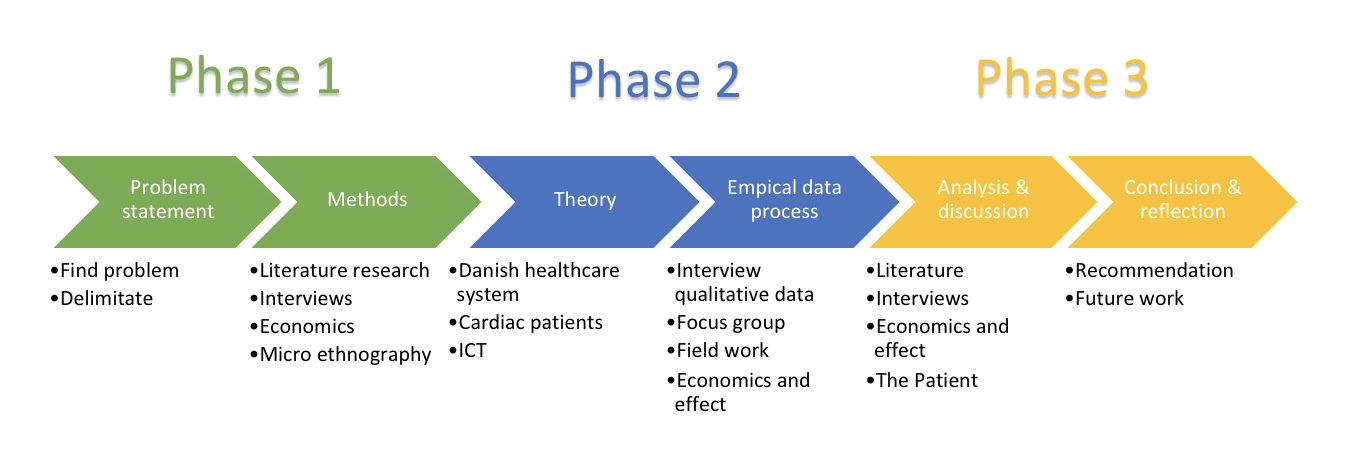
\includegraphics[width=1.10\textwidth]{Figure/researchdesign.png}
\caption{Research design}
\label{fig:Researchdesign}
\end{figure} 

\Cref{fig:Researchdesign} is an overview of the research design in this paper.
 Phase 1 in the study is the initial process, phase 2 is knowledge/data process and phase 3 presents the analysis and outcome.
In phase 1 the topic was selected and translated into questions and hereby the problem statement. In this process the delimitation of the project was laid out. Furthermore the methodology was chosen during this fase in the project. The methodology contains considerations in literature search, interview method and data analyzing methods. 
Phase 2 is the process to gain knowledge and collect the necessary data to analyze the problem. The knowledge is gathered through a literature search in the area. The method is described in \Cref{literature}. The data is collected throughout interviews with both cardiac patients and a research nurse. To learn more about the interview and the empirical process read \Cref{qualitative} and \Cref{empirical}.
In phase 3 the collected data and knowledge is analyzed and evaluated. Furthermore the newly gathered information are discussed within the literature search. The closing statement in this study will be an overall conclusion of the studies findings. The last process in the project is to reflect and look into further investigation of the problem. 


\section{Literature search method}
\label{literature}

The literature was conducted with a thorough literature research. To find the right type of literature PICO (Population/Problem, Intervention, Comparison/Control, Outcome) was used as a framework, see \Cref{PICO} \cite{pico}. 
Following databases have been used for this project: PubMed,  AUlibrary, Embase and google scholar.
The literature search started in february 2018, where the primary part of the literature was collected within two month, although literature has been collected through the hole period of the writing process. 
Search keywords was conducted in the problem statement and have been used for search words in the databases. Following words was chosen as key words: ICT, Healthcare, cardiovascular, rehabilitation, cost effectiveness.
The papers were chosen from title and abstract. Furthermore, other literature was conducted through chain search found in relevant literature. Multiple papers was deselected due to irrelevance or mismatch of the subject. The national guidelines and national history was conducted on state webpages. The keywords were combined with an "AND" - and in related areas an "OR". The PICO blocks was as well combined with the "And" and "OR". Furthermore, a search criteria was compiled in relation to the publication year of the paper.  Therefore, most of the literature used in this project is no more than 10 years old. This restriction was made as a lot of research has been made in the area of telemedicine, and to achieve the best result it is important to use the most recent knowledge within this area. 

\begin{table}[H]
\begin{longtabu} to \linewidth{@{}l l X[j]@{}}
    \textbf{PICO} &        \textbf{Search headings} \\[-1ex]
    \midrule
     Population/Problem:   &    Patients with cardiac illness \\ \hline
    Intervention:   &        Patient in telerehabiliation \\ \hline
    Comparison/Control:    &        Standard cardiac rehabilitation \\ \hline
    Outcome:    &        Adherence to CR, readmission, mortality 
    \newline
   \end{longtabu}
\caption{Search headings in PICO principles \cite{pico}}
\label{PICO}
\end{table}



\section{Research interviews}
\label{qualitative}

Research interviews are defined as a purposeful conversation between two or more people, whereas an interviewer ask concise and unambiguous questions and the interviewee will respond. To collect data for this study interviews with experts within rehabilitation of  cardiac patients and cardiac patients themselves has been made \cite{mark2009research}. 

There are many types of interviews, but for this study a Semi-structured interview has primarily been used. The semi-structured interviews can be exploratory, explanatory and evaluative. Furthermore, this kind of interview is referred to as qualitative research interviews.
This type of interview makes it possible to prepare the interviews setup, but it also allow the interviewee to expand the knowledge area end hereby expand the outcome of the interview. 
Besides the expansion of the frame this setup allows the interviewee to explain the opinions and reasons for attitude. Semi-structured interviews provide the opportunity to probe answers whereas the interviewee can explain their responses. The interview may also lead the discussion into unforeseen areas, which can collaborate to new knowledge. The different interview types gives a detailed set of data, but it can be viewed as biased due to the interviewers impact on the interviewee. Using semi-structured interviews allowed us to gain insight on the use of telerehabilitation in CR from different point of views which will benefit our analysis.

In this project the questions are formed as open ended and only as a frame, hence the semi-structured interview \cite{mark2009research}.

To prepare for the semi-structured interviews the "five p's" were used: Prior, Planning, Prevents, Poor and Performance. To withhold these p's following was taken into account. Level of knowledge, developing the interview themes, inform interviewee before interview and finding an appropriate location. 

The group had gained a lot of prior knowledge about the rehabilitation process of cardiac patients in Denmark. This supports the capability to accurate response under the interview and the interviewers credibility. The knowledge was secured during the literature research fase \cite{mark2009research}. 

For the interviews hold with experts in rehabilitation of cardiac patients, the interview questions were designed to make sure that every area wanted to be clarified was conducted. Ideas to make relevant questions came from literature and the problem statement. The prepared questions are present in app XXX. The frame made for these interviews was made as a guide in a perhaps logical order. The location of the interview should be convenient for the partipant otherwise they might feel uncomfortable which could impact the data collection. For these interviews the participants chose the location to oblige convenience for the participant. 

\section {Focus group/open discussion with patients} \label{focusgroup}

A focus group is defined as an interview method that involves more than one but usually at least four participants. The interview takes place in a fairly unstructured setting. The person who runs the interview is the moderator or facilitator and is expected too guide the session without being intrusive. In this paper the focus group session was held with the patients who attends the CR in Herning Municipality at that moment. The data collection from this focus group is qualitative and is used to collect the opinion on ICT used in rehabilitation of cardiac patients. This setup gives the researchers the possibility to understand the way people feel. The set up also gives opportunity for the attendies to probe each other \cite{brymanbell}. 

The questions for the focus group was premade and pointed for the group of patients. The short focus group was held in continuation of the education and training class. This means that the participants had a knowledge of the project and project members.
Through the interview both premade and new question was asked during the session. The interview was recorded and transcribed, the transcription can be seen in APP XXXX. The session is further described in \Cref{patientinterview}. 

\section{Micro ethnography} \label{ethnography}
The method ethnography is used when an observer/ethnographer immerses in a group for an extended period. For this project it has not been possible to follow the CR in Herning Municipality for an extended period. However, a micro ethnography has been carried out. The project group attended a training and education session for cardiac patients in Herning Municipality. The participant observer role is classified in four role types: \textit{Complete participant}, \textit{Participant-as-observer}, \textit{Observer-as-participant} and \textit{Complete observer}. For the training and education session in Herning Municipality the researchers attend in the role as \textit{Participant-as-observer}. The \textit{Participant-as-observer} is a fully functioning member in the setting and the social setting is aware of the researchers status as a researcher \cite{gold1958roles}. The purpose of the participation is to connect with the patients before the focus group and to the get a sense of the social setting in the cardiac rehabilitation. During the session mental field notes were taken. The notes was taken as mental notes where as much as possible is remembered during the session and written down later. This is a method that results in a low detail level, but it makes it possible to fully participate within the session without interferring with social setting \cite{lofland1995analyzing}. This field work was prior to the focus group/open discussion with the patients and that might make the patients feel more comfortable sharing their thoughts. The Field notes can be read in app XXXX. 

\section{Analyzing qualitative data}

Qualitative research is depending on social interaction and therefore the qualitative data is analyzed in an interactive and iterative process. Qualitative data are likely to be more varied, elastic and complex than quantitate. An analyzing method is therefor a great tool to evaluate and use the data to answer the research questions. 

To analyze the data from the semi-structured interviews an analyzing tool was necessary. The Narrative analysis method has been chosen to perform this process. The narrative analysis consist of a collection of different approaches to analyse qualitative data. 

The study only have the narrative of a few individuals, but they are able to give another perspective within the healthcare system than what is stated in literature. The interviews gave the opportunity to look into a small peace of the Danish Healthcare System, more likely region Midtjylland and specific Herning Municipality. With the narrativ analysis of the qualitative data it was possible to analyze themes to compare the narrators opinion on the use of telerehabilitation in centre based CR \cite{mark2009research}. 

  

\section{Economy}

Various approaches are possible when evaluating and comparing a technology to the existing method. For this study one approach has been chosen to look into the cost and effect of telemedicine rehabilitation in Denmark.

\subsection{Cost-effectiveness analysis}

When implementing new technology and rehabilitation processes, it is important to look at the cost. Every region and municipality are on a budget which is provided by the state. Therefore, resource allocation is a big part of the Danish system. In healthcare, cost is not the only value which is taken into account, the patients’ health and well-being is an important part of the puzzle. When allocating money for one intervention, another intervention may be dismissed. This is why a decision tool is needed to evaluate interventions and pick the interventions that provides the most benefit with the available resources.

Cost-Effective Analysis (CEA) is an analysis of cost and effectiveness of perhaps a new service or technology. The benefit by using a CEA is that it does not only look into cost but also takes the patient into account. It is often used to evaluate effectiveness in healthcare. In this study the CEA is used to compare the traditional CR with the new setup where tele rehabilitation is used. Incremental Cost-Effectiveness Ratio (ICER) is a type of CEA and is used to analyse healthcare interventions. Therefore, this analysis tool has been used in this study. In the analysis the CE ratio is calculated. The CE ratio is the cost associated divided with health outcome \cite{bang2012median}.

The data for the analysis is collected in corporation with Herning Hospital and Herning Municipality. 

Following costs are taken into account:


\begin{longtabu} to \linewidth{@{}l X[j] @{}}
	\textbf{Health related} & \textbf{Non-health related}\\[-1ex]
	\midrule
	Profession (Staff) & (Travel) \\[-1ex]
	Rehospitalization & (Productivity loss) \\[-1ex]
	Physical materials & (Presentism loss)\\[-1ex]
	Training equipment &  \\[-1ex]
	Other cost &  \\[-1ex]
	(Medication) &  \\[-1ex]
	IT &  \\[-1ex]
	\hline
	\caption{Cost variables CEA}
\end{longtabu}

The different costs in this setup can vary at lot from municipality to municipality and furthermore in between countries. Moreover, the choice of the cost taken into count. The selected costs in this project is chosen due to research in similar trials and the cost possible to be collected \cite{costeffect, usingeffect}. 

Following costs has been left out of the analysis: Travel reimbursement, Productivity loss, Presentism loss and Medication. The mentioned costs are all a part of evaluating a health technology as this, but not possible to collect in this study. Travel reimbursement is left out because it is a cost for the patient and not for the municipality. Productivity loss is left out because the average cardiac patient is above or about the pension age. Medication is a big area and would definitely be an interesting element to include. Unfortunately, this is an area that is too big and would require a greater effort as to what is possible in this project. Therefore, it is not possible to collect the needed data within the medication area. \\

The measure of effect can be done in various scale methods. For this project quality-adjusted life year (QALY) has been chosen. "The QALY is able to combine ‘the effects of health interventions on mortality and morbidity into a single index’, thereby providing a ‘common currency’ to enable comparisons across different disease areas" \cite{QALY}. This evaluation method combines survival with health-related quality of life (HRQoL). QALY is an index between 1 and 0 and the higher the QALY index is the better the effect of the intervention. The QALY methods makes it easier to look at both the patients personal experience and medical facts \cite{QALY}. To obtain the data from the patient an EQ-5D questionnaire can be used \cite{costeffect}. This study will not perform any actions to obtain a QALY index, but the data will be obtained from literature with similar studies where the QALY index haven been measured and calculated with the EQ-5D questionnaire.








